In the next section this theorem is used to show the existence of the relative Deligne tensor product. The existence of the relative Deligne tensor product is essential for the construction of the symmetric monoidal 3-category of tensor categories: it provides the composition of 1-morphisms. This is the primary reason that all our tensor categories are assumed to be rigid. Rigidity also plays a role in the theory of exact module categories described in the section~\ref{sec:tc-exact}.

Without assuming that the category is rigid, the conditions of the theorem \ref{thm:C-module-Embedding} are absolutely necessary. In fact without rigidity theorem \ref{thm:EGNO2.11.6} above fails as the following example shows: 

\begin{example} \label{ex:lax-module}
	Let $\cR \cong \Vect \oplus \Vect \cdot X$ be the non-rigid linear monoidal category consisting of pairs of vector spaces, which we write as $V_1 + V_2 X$, with tensor product given by 
	\begin{equation*}
		(V_1 + V_2 X) \otimes (W_1 + W_2 X) = V_1 \otimes W_1  +  (V_1 \otimes W_2 \oplus V_2 \otimes W_1)X.
	\end{equation*} 
	Up to equivalence there are unique choices of associator and unitors making this a linear monoidal category. 
It is both finite and semisimple, and is a categorification of the ring $k[x]/(x^2)$, but it is not rigid. The object $X$ cannot have a dual as there is no object $Z \in \cR$ such that $Z \otimes X$ has a non-zero map to or from the unit object of $\cR$. 
	
	There is a tensor functor $F:\cR \to \Vect$ given by $(V_1 + V_2 X) \mapsto V_1$. This gives the category $\Vect$ the structure of a (left) $\cR$-module category, and moreover $F$ is naturally an $\cR$-module map. $F$ has both left and right adjoints, which agree and are given by the functor $G: \Vect \to \cR$ sending $W \in \Vect$ to $(W + 0 X) \in \cR$. It is not possible to give $G$ the structure of a (strong) $\cR$-module functor. Moreover there is no algebra object $A \in \cR$ such that $\Vect$ is equivalent to $\Mod{}{A}(\cR)$ as linear categories, let alone as $\cR$-module categories. 
\end{example}

\begin{proof}
	 By Theorem \ref{thm:EGNO2.11.6}, there exist algebra objects $A, B \in \cC$ and equivalences $\cM \simeq \Mod{A}{}(\cC)$ and $\cN \simeq \Mod{}{B}(\cC)$. By Lemma \ref{lma:RigidIsExact}, the natural tensor product functor
	\begin{equation*}
		\cM \times \cN \simeq \Mod{A}{}(\cC) \times  \Mod{}{B}(\cC) \to \Mod{A}{B}(\cC)
	\end{equation*}
	is exact in each variable separately. It is also $\cC$-balanced. Thus $(2)$ implies both  $(1)$ and $(3)$. We will first prove (2), and then establish (4).  We wish to show that for any $\cD$ the category of right exact functors 
\begin{equation*}
	\overline{F}:\Mod{A}{B}(\cC) \to \cD
\end{equation*}
	is naturally equivalent to the category of $\cC$-balanced functors $F:\cM \times \cN \to \cD$ which are right exact in each variable separately. It is clear that every functor of the former type restricts to one of the later type, and so we must show that a functor of the later types extends uniquely (up to canonical isomorphism) to one of the former type. 
	
The key insight is to note that every object of $X \in \Mod{A}{B}(\cC)$ may be functorially written as a coequalizer of objects in the image of $\cM \times \cN$. For example we have:
\begin{equation*}
	{}_A A \otimes A \otimes X_B \rightrightarrows {}_A A \otimes X_B \to {}_A X_B.
\end{equation*}
Let $\delta: {}_A A \otimes A \otimes X_B \to {}_A A \otimes X_B$ be the difference map. 
For any right exact functor $\overline{F}$, the value $\overline{F}({}_A X_B)$ is canonically determined as a cokernel:
\begin{equation*}
	\overline{F}({}_A X_B) = \coker \left( \overline{F}(\delta): \overline{F}({}_A A \otimes A \otimes X_B) \to \overline{F}({}_A A \otimes X_B) \right).
\end{equation*} 
Moverover the modules ${}_A A \otimes A \otimes X_B$ and ${}_A A \otimes X_B$ are in the image of $\cM \times \cN$. 
	
Suppose we are given a $\cC$-balanced functor $F:\cM \times \cN \to \cD$ which is right exact in each variable separately. It is tempting to try to define the extension $\overline{F}: \Mod{A}{B}(\cC) \to \cD$ via a formula of the type:
\begin{equation*}
	\overline{F}({}_A X_B) := \coker \left( \underbrace{{F}(\delta)}_{\textrm{what is this?}}: F({}_A A \otimes A,  X_B) \to {F}({}_A A , X_B) \right).
\end{equation*} 
If this were possible, then it would immediately follow that the extension $\overline{F}$ is determined (up to unique natural isomorphism) by its restriction to $\cM \times \cN$, and that, moreover, the category of $\cC$-balanced exact-in-each-variable functors $F:\cM \times \cN \to \cD$ is equivalent to the category of functors  
$\overline{F}: \Mod{A}{B}(\cC) \to \cD$.

However it is not possible to define $\overline{F}$ in this way, at least not immediately. The difficulty is that while the relevant objects are in the image of $\cM \times \cN$, the map $\delta$ is not. 
Yet for each $X \in \Mod{A}{B}(\cC)$ we may form the commutative diagram\footnote{The fact that this diagram commutes uses the coherence and naturality of the $\cC$-balanced structure. To verify the commutativity it is easiest to break each difference map into its constituent piece (one from the multiplication in either $A$ or $B$, and one from the action on $X$) and to show commutativity with respect to these maps.} shown in Figure \ref{fig:RelDelingePdtDiagram}.
\begin{figure}[htbp]
	\begin{center}
		\begin{tikzpicture} \matrix (m) [matrix of math nodes, row sep={1.5cm,between origins}] {
		 F({}_AA \otimes A \otimes X, B \otimes B_B) &[1cm] F({}_AA \otimes X, B \otimes B_B) &[1cm] F({}_A X, B \otimes B_B) &[0.5cm] 0 \\
		F({}_AA \otimes A, X \otimes B \otimes B_B) & F({}_AA, X \otimes B \otimes B_B) & & \\
		F({}_AA \otimes A, X \otimes B_B) & F({}_AA , X \otimes B_B) & & \\
		 F({}_AA \otimes A \otimes X, B_B) & F({}_AA \otimes X, B_B) & F({}_AX,B_B)  & 0 \\
		& &\overline{F}({}_AX_B)  & \\
			};
			\draw [->] (m-1-1) -- node [above] {$\delta_1$} (m-1-2);
			\draw [->] (m-1-2) -- node [above] {$$} (m-1-3);
			\draw [->] (m-1-3) -- node [above] {$$} (m-1-4);
			\draw [->] (m-4-1) -- node [above] {$\delta_1$} (m-4-2);
			\draw [->] (m-4-2) -- node [above] {$$} (m-4-3);
			\draw [->] (m-4-3) -- node [above] {$$} (m-4-4);
			\draw [->] (m-1-1) -- node [left] {$\cong$} (m-2-1);
			\draw [->] (m-1-2) -- node [left] {$\cong$} (m-2-2);
			\draw [->] (m-3-1) -- node [left] {$\cong$} (m-4-1);
			\draw [->] (m-3-2) -- node [left] {$\cong$} (m-4-2);
			\draw [->] (m-2-1) -- node [left] {$\delta_2$} (m-3-1);
			\draw [->] (m-2-2) -- node [left] {$\delta_2$} (m-3-2);
			\draw [->,dashed] (m-1-3) -- node [left] {$\overline{\delta}_X$} (m-4-3);
			\draw [->,dashed] (m-4-3) -- node [left] {$$} (m-5-3);
			\node [node distance = 1.75cm, left of= m-5-3] {$\coker(\overline{\delta}_X)=:$};
		\end{tikzpicture}
	\end{center}
	\caption{A digram useful for demonstrating the existence of the relative Deligne tensor product.}
	\label{fig:RelDelingePdtDiagram}
\end{figure}
Here the arrows labeled with isomorphisms come from the $\cC$-balanced structure of the functor $F$, while the remaining solid arrows are maps in the image of $\cM \times \cN$. The maps labeled with either $\delta_1$ or $\delta_2$ represent difference maps, as above. 

The rows of this diagram are exact (since $F$ was assumed to be right exact in each variable) and hence this diagram defines a unique map $\overline{\delta}_X$, shown as the long dashed arrow in the diagram. This is precisely the missing map, and hence we may define the value of the extension $\overline{F}$ on the object ${}_AX_B$ as the cokernel of $\overline{\delta}_X$. We leave it to the reader to verify that this extension gives a well-defined right exact functor 
\begin{equation*}
	\overline{F}: \Mod{A}{B}(\cC) \to \cD,
\end{equation*} 
and implements the desired equivalence between such right exact functors and $\cC$-balanced exact-in-each-variable functors. Verifying that this construction is well defined makes use of the pentagon identity satisfied by $\cC$-balanced functors. This establishes (1), (2), and (3). The final property, part (4), now follows from a routine diagram chase, which we also leave to the reader. 
%\CSPcomm{old material...}	
%Thus every right exact functor and every natural transformation between such functors is determined by its restriction to $\cM \times \cN$. Conversely every $\cC$-balanced functor $F: \cM \times \cN \to \cD$ gives rise to a functor $\overline{F}: \Mod{A}{B}(\cC) \to \cD$; its value on ${}_A X_B$ is defined as the coequalizer:
%\begin{equation*}
%		\overline{F}({}_A X_B) := \coeq \left(  F({}_AA \otimes A, X_B) \rightrightarrows F({}_A A, X_B) \right).
%\end{equation*}
%This establishes (1), (2), and (3).
% To see that the value on natural transformations is determined we can observe that there is a funcotial splitting of F(A, X) \to F(X)  as B-modules (not as A-B bimodules). This is enough to establish that the natural transformation is derimined by its values on $\cM \times \cN$.
%Part (4) is a standard exercise. 
\end{proof}

%\begin{remark} \label{rmk:rigidpreservedbytensor}
%	We may use the case $\cC= \Vect_k$ to rewrite part of the data of a tensor category as a linear category $\cD$ equipped with an object $1 \in \cD$ and a linear functor $\otimes: \cD \boxtimes \cD \to \cD $, together with natural transformations $\alpha$, $\lambda$, and $\rho$, as before. Moreover by Corollary \ref{cor:RigidityViaFunctors} the tensor product of two rigid tensor categories is again rigid. 
%\end{remark}

\begin{remark}
	If ${}_{\cD}\cA_{\cC}$ and ${}_{\cC}\cB_{\cE}$ are bimodule categories, then the actions of $\cD$ and $\cE$ induce a $\cD$-$\cE$-bimodule category structure on $\cA \boxtimes_{\cC} \cB$. This bimodule category satisfies the analogous universal property for $\cC$-balanced bilinear bimodule functors. 
\end{remark}

\begin{remark}
The above theorem assumes that $\cC$ is a tensor category, that is a finite rigid linear monoidal category.  The finiteness assumption is probably not essential, though it certainly simplifies the proof of the existence of the relative Deligne tensor product.  It would be worthwhile to have interesting non-finite examples to motivate extending our results to more general linear categories.
\end{remark}
\CD{Add comment on importance/essentialness of right exactness in the theorem?}




In \cite{0909.3140} the existence of the relative Deligne tensor product was established for semisimple module categories over semisimple tensor categories over a field of characteristic zero. The following theorem extends these results and provides an alternative proof of the existence of the relative Deligne tensor product.   


The following is an elaboration of results of \cite{MR1976459} and \cite{EO-FTC}. % Really: enriched is due to EOFTC sec 3.2 (Ost03 did the semisimple case), the rest is new.
\begin{proposition} \label{thm:enrichment-of-mod-cats}
	Let $\cC$ be a finite linear monoidal category and let $\cM$ be a finite $\cC$-module category. Then $\cM$ is enriched, tensored, and cotensored over $\cC$ with the tensor structure coming from its structure as a $\cC$-module category.
\end{proposition}

\begin{proof}
	What this means is that there exist functorial assignments of objects $\IHom(m', m) \in \cC$ and $(m^c) \in \cM$ for every $m,m' \in \cM$ and $c \in \cC$ and natural isomorphisms
	\begin{equation*}
		\Hom_\cC(c, \IHom(m', m)) \cong \Hom_\cM(c \otimes m', m) \cong \Hom_\cM( m', (m^c))
	\end{equation*}
	witnessing adjunctions
	\begin{equation*}
			c \otimes (-) \quad \dashv\quad (-^c) \quad \textrm{ and } \quad (-) \otimes m' \quad \dashv \quad \IHom(m', -).
	\end{equation*}
Such structure exists precisely if the functors
\begin{align*}
	\Hom_\cM((-)\otimes m', m): \; & \cC^\op \to \Vect \\
	\Hom_\cM(c \otimes (-), m): \; & \cM^\op \to \Vect
\end{align*}
are representable. In this case they represent the objects $\IHom(m', m)$ and $(m^c)$, respectively. Both of these functors are left exact, and hence by Lemma \ref{lma:left_exact=linear} (which uses the finiteness of $\cC$ and $\cM$) both of these functors are indeed representable. 
\end{proof}

\begin{remark}
	The existence of $\IHom(m', m)$ only requires $\cC$ to be finite, and similarly the existence of $(m^c)$ only requires $\cM$ to be finite.
\end{remark}


\begin{definition}
	Let $\cC$ be a finite linear monoidal category and let $\cM$ be a finite $\cC$-module category. An object $p \in \cM$ will be called {\em $\cC$-projective} if $\IHom(p, -)$ is right exact (it is automatically left exact). An object $p$ will be called a {\em $\cC$-generator} if $\IHom(p,-)$ is faithful. % \NS{Are you assuming rigidity here?}
\end{definition}

\begin{remark}
	An object $p \in \cM$ is a $\cC$-generator if and only if for each object $x \in \cM$ there exists an object $c \in \cC$ and a surjection $c \otimes p \twoheadrightarrow x$ if and only if for each object $x \in \cM$ the canonical map $\IHom(p,x) \otimes p \twoheadrightarrow x$ is a surjection. In particular an ordinary generator (i.e. an object such that $\Hom_\cM(p,-)$ is faithful) is also a $\cC$-generator. 
\end{remark}

\begin{example} \label{ex:rigid_all_C-proj}
	Let $\cC$ be a tensor category, i.e., $\cC$ is both finite and rigid. We may view $\cC$ as a left $\cC$-module category over itself. Since $\cC$ is rigid, we have isomorphisms $\IHom(x,y) \cong y \otimes x^*$ and $(y^x) \cong {}^*x \otimes y$. Moreover Lemma \ref{lma:RigidIsExact} states that in this case the tensor product is exact in each variable, hence {\em every object} of $\cC$ is $\cC$-projective, even if the object is not a projective object in the usual sense. %\NS{To use that lemma you need to assume rigidity.}
\end{example}




We will follow the standard conventions for bicategories and their functors, as in for example \cite{MR2664622}. In particular for every pair of composable 1-morphism in a bicategory, 
\begin{itemize}
	\item a {\em lax} functor of bicategories $F: \cB \to \cC$ is equipped with natural 2-morphisms
	\begin{equation*}
		F(f) \circ F(g) \to F(f \circ g) \quad \textrm{ and } \quad \id_{F(X)} \to F(\id_X);
	\end{equation*} 
	\item an {\em oplax} functor of bicategories $F: \cB \to \cC$ is equipped with natural 2-morphisms
	\begin{equation*}
		F(f \circ g) \to F(f) \circ F(g)   \quad \textrm{ and } \quad F(\id_X) \to \id_{F(X)}; and
	\end{equation*}
	\item a {\em strong} functor of bicategories the comparison maps are 2-isomorphisms (hence a strong functor may be regarded as both lax and oplax). 
\end{itemize}

\begin{definition}
	Let $\cC$ and $\cD$ be tensor categories. A {\em $\cC$-$\cD$-bimodule category} is a bicategory with two objects $x$ and $y$ such that
	\begin{itemize}
		\item all hom categories are linear categories, 
		\item horizontal composition is multilinear, and
		\item the hom categories $\Hom(x,x)$, $\Hom(y,y)$, and $\Hom(y,x)$ are respectively $\cD$, $\cC$, and empty.
%		there are identifications of monoidal categories $\Hom(x,x) = \cD$ and $\Hom(y,y) = \cC$, and the set $\Hom(y,x)$ is empty.
	\end{itemize}
	We will often abuse notation and refer to the value $\cM = \Hom(x,y)$ as the bimodule category. If $\cD \simeq \Vect_k$, then $\cM$ is called a {\em left $\cC$-module category}. If $\cC \simeq \Vect_k$, then $\cM$ is called a {\em right $\cD$-module category}.
\end{definition}
	
Unwrapping this definition we see that a


\begin{lemma} \label{lma:RigidIsExact}
	Let $(\cC, \otimes)$ be a tensor category (so that $\cC$ is rigid). Then the multilinear functor $\otimes: \cC \times \cC \to \cC$ is exact in both variables. 
\end{lemma}

\begin{proof}
	The units and counits give rise to natural isomorphisms %\NS{Currently we have both $\Hom$ and $\Hom$ in the paper.  We should pick one.}
 \begin{equation*} 
 	\Hom(x \otimes y, z) \cong \Hom( x, z \otimes y^*) \cong \Hom(y, {}^*x \otimes z).
 \end{equation*}
	Hence for all $x$ and $y$ the functors $(-)\otimes x$ and $y \otimes (-)$ admit both left and right adjoints, and are consequently exact. 
\end{proof}

\noindent In particular we have the following sequences of adjunctions:
\begin{alignat*}{5}
	& x^* \otimes (-)  \quad & &  \dashv \quad &&  \quad x \otimes (-)  \quad &&  \dashv &&  \quad {}^*x \otimes (-), \\
	& (-) \otimes {}^* y  \quad & &  \dashv \quad &&  \quad (-) \otimes y  \quad &&  \dashv &&  \quad (-) \otimes y^*. 
\end{alignat*}

\begin{corollary}
	A tensor category $\cC$ is semisimple if and only if $1 \in \cC$ is a projective object. 
\end{corollary}
%\CD{semisimple hasn't yet been introduced}
%\CSP{We are not writing a text book. We don't have to define semisimple.}

\begin{proof}
	If $\cC$ is semisimple then every object is projective, so in particular the unit object is projective. Conversely, if $1 \in \cC$ is projective, then $\Hom(P, -) = \Hom( 1, (-) \otimes P^*)$ is an exact functor for all $P$. Hence every object is projective, and it follows that $\cC$ is semisimple.  
\end{proof}

\begin{lemma}
	The assignments $x \mapsto x^*$ and $x \mapsto {}^*x$ gives rise to equivalences of tensor categories $(-)^*: \cC \to \cC^{mop}$ and ${}^*(-): \cC \to \cC^{mop}$. Consequently the assignment $x \mapsto x^{**}$ gives an autoequivalence of any tensor category. 
\end{lemma}

%\begin{proposition}
%If $\cC$ is a fusion category, then there exist monoidal functors $\ld{(-)} : \cC \ra \cC^{\mop}$ and $\rd{(-)} : \cC \ra \cC^{\mop}$ whose values on any object $a \in \cC$ are respectively a left dual object $\ld{(a)}$ and a right dual object $\rd{(a)}$ for $a$.
%\end{proposition} \CD{This proposition doesn't actually depend on fusion, right?  Should change the statement so that only what is needed (existence of duals) is assumed.}

\begin{proof}
Let $\otimes$ denote the tensor product on $\cC$ and $\cdot$ the tensor product on $\cC^{\mop}$, so that $x \cdot y = y \otimes x$.

First we construct the functor ${(-)^*}$.  Define ${(-)^*}$ on objects by picking for each object $a \in \cC$ a right dual object ${a^*} \in \cC$.  Also pick a unit map $\eta_a: 1 \ra a \otimes {a^*}$ and a counit map  $\varepsilon_a: {a^*} \otimes a \ra 1$  giving ${a^*}$ the structure of a right dual to $a$.  Define the functor ${(-)^*}$ on a morphism $f: a \ra b$ to be its {\em mate}: 
\begin{equation*}
	{(f)^*} := (\varepsilon_b \otimes \id_{\rd{a}}) (\id_{\rd{b}} \otimes f \otimes \id_{\rd{a}}) (\id_{\rd{b}} \otimes \eta_a).
\end{equation*}

Next we want to construct a monoidal functor structure on $(-)^*$, that is we need natural transformations $f_{a,b}: (a \otimes b)^* \rightarrow a^* \cdot b^* = b^* \otimes a^*$.  Since the right dual is unique up to unique isomorphism, it is enough to check that $b^* \otimes a^*$ is a right dual to $a \otimes b$.  Observe that the morphisms $\rd{b} \otimes \rd{a} \otimes a \otimes b \xra{\varepsilon_a} \rd{b} \otimes b \xra{\varepsilon_b} 1$ and $1 \xra{\eta_a} a \otimes \rd{a} \xra{\eta_b} a \otimes b \otimes \rd{b} \otimes \rd{a}$ show that $(\rd{b} \otimes \rd{a})$ is a right dual to $(a \otimes b)$.  There is therefore a uniquely determined isomorphism from $(\rd{b} \otimes \rd{a})$ to $\rd{(a \otimes b)}$.  It is straightforward to check that this isomorphism is natural and defines a monoidal functor.
The left dual functor is analogous, and is easily seen to be the quasi-inverse of the right dual functor. 
%Since the left and right duals are quasi-inverse to each other, they're each equivalences.
% In principle, need to check naturality and hexagon for those isos.
\end{proof}
\begin{remark}
Applying this theorem to $\cC^{\op}$ shows that the left dual and the right dual each give monoidal equivalences between $\cC^{\op}$ and $\cC^{\mp}$.  Nonetheless, these equivalences are not canonical (indeed we have exhibited two natural choices), so we will always be careful to distinguish  $\cC^{\op}$ and $\cC^{\mp}$.
\end{remark}

%\CSP{Do we need this last cor?}
%\begin{corollary} \label{cor:RigidityViaFunctors}
%	A tensor category $(\cC, \otimes, 1)$ is rigid if and only if there exists an equivalence of tensor categories ${{}^*(-)}: \cC \to \cC^\mp$ and natural isomorphisms
%	\begin{align*}
%		\Hom( {}^*y, z) &\cong \Hom(1, z \otimes y) \\
%		\Hom(z, y) & \cong \Hom(z \otimes {}^*y, 1).
%	\end{align*}
%\end{corollary}
%
%\begin{proof}
%	It is clear from the previous lemma that a rigid tensor category admits such a structure (the natural isomorphisms in question are induced by the evaluation and coevaluation). Conversely, if we are given such a structure, then applying the above natural isomorphisms in the cases $z={}^*y$ and $y$ yield evaluation and coevaluation maps demonstrating ${}^*y$ as the left dual of $y$. Right duals are obtained by the same argument applied to the inverse of the functor ${}^*(-)$.
%\end{proof}
%
%% This fact is asserted in Bruce's thesis; the functor part is mentioned in Selinger Eg 4.4.


%\begin{remark}
%The monoidal functor $\ld{(-)}: \cC \ra \cC^{\mop}$ is an equivalence of tensor categories; the inverse functor is $\rd{(-)}: \cC^{\mop} \ra \cC$.
%\end{remark}


%Consider the following example:
%\begin{example}
%	For any category $\cA$, the functor category $\Fun(\cA, \cA)$ is a monoidal category with tensor product given by composition of functors $\circ$. 
%\end{example}


%We impose one further convention (Convention (C)), which is that Convention (A) and Convention (B) should hold simultaneously in the above example. This forces us to consider the object $x^*$ as the {\em left adjoint} (or {\em left dual}) of $x$, despite the fact that the ``$*$'' occurs on the right of the symbol ``$x$''. 

%\NScomm{[Note that there is another option.  In order to interpret $x^*$ as an adjoint, we need to interpret $x$ as a morphism and $\otimes$ as composition.  As always there are competing conventions about whether $f \otimes g$ means $f(g(-))$ or $g(f(-))$.  We were implicitly using the former convention.  If you use the latter then Conventions (A) and (B) hold, and then $x^*$ is a right dual as in EGNO and ENO.  We plan to change to this latter convention in the next reversion of the paper.]}

%This has the following natural consequences:
%\begin{itemize}
%	\item The left dual acts on the left of the object $x$ to produce a map to the unit. 
%	\item These notions extend to duals for the 2-category $Alg$ of algebras, bimodules, and bimodule maps: An $A$-$B$-bimodule $M$ with a left adjoint (or left dual) ${}_BM^L_A$ has evaluation and coevaluation maps:
%	\begin{equation*}
%		ev: {}_BM^L \otimes_A M_{B} \to {}_B B_B, \quad \quad coev: {}_AA_A \to {}_A M \otimes_B M^L_A.
%	\end{equation*}
%	\item Thus an $A$-$B$-bimodule should be considered a morphism from $B$ to $A$, for then there is a functor $Alg \to \Cat$ sending an algebra $A$ to its category $\Mod{A}{}$ of left modules, which sends left duals to left adjoint functors, and similarly for right duals. 
%	\item Moreover way we typically write composition of bimodules then agrees with the way we write composition of their corresponding functors. 
%\end{itemize}

%If one insists on the opposite convention, calling $x^*$ the right dual of $x$, then one must also deny Convention (C) and these consequences. We end with a final well-known observation. 

% This remark is no longer needed.
%\begin{remark}
%	Suppose $x$, an object of a monoidal category, admits a right dual.  There is a category whose objects $(x^*, \eta, \varepsilon)$ consist of right duals to $x$, with compatible choices of unit and counit maps. This category is contractible (equivalent to the terminal category). Hence the choice of a right dual is unique up to unique isomorphism. In particular there are canonical isomorphism ${}^*(x^*) \cong ({}^*x)^* \cong x$. 
%The same observation applies to adjoint functors, adjoints of bimodules, and generally to any adjoint in any 2-category.  
%\end{remark}


\section{Module categories}

\subsection{Module categories are categories of modules}

The following is an extension of \cite[Thm 2.11.2]{EGNO} and \cite[Thm 1]{MR1976459}.

\begin{theorem} \label{thm:C-module-Embedding} %!% [Thm 2.11.6(i)] 
	Let $\cM$ be a finite left module category over a finite, but not necessarily rigid, linear monoidal category $\cC$. Fix an object $p \in \cM$, and set $A = \IHom(p,p) \in \cC$. The object $A$ is naturally an algebra object in $\cC$, and gives rise to $\cC$-module functor:
	\begin{align*}
		F:   \Mod{}{A}(\cC) \to \cM \\
		F(x_A) := \coeq \left( x \otimes \IHom(p,p) \otimes p \rightrightarrows x \otimes p \right).
	\end{align*}
The functor $\IHom(p,-): \cM \to \Mod{}{A}(\cC)$ is right adjoint to $F$. 

Assume that $\IHom(p,-)$ may be equipped with the structure of a $\cC$-module functor and that the unit and counit of the adjunction $F \dashv \IHom(p,-)$ are morphisms of $\cC$-module functors. Assume further that $p$ is a $\cC$-projective $\cC$-generator.  Then the $\cC$-module adjunction  $F \dashv \IHom(p,-)$
	induces an equivalence of left $\cC$-module categories $\cM \simeq \Mod{}{A}(\cC)$. 
\end{theorem}

\noindent The proofs given in \cite{EGNO} and \cite{MR1976459} at first appear to depend on  the rigidity of the tensor category $\cC$. Indeed the first step of the proof of \cite[Thm 2.11.2]{EGNO} invokes \cite[lemma 2.10.4.(4)]{EGNO} whose proof makes explicit use of rigidity. The same lemma is used in step (3) of the proof of \cite[Thm 1]{MR1976459}. However with a little care this is easily avoided (cf. \cite[Rmk. 2.11.3]{EGNO}). 

The Barr-Beck monadicity theorem implies that $\cM$ is equivalent to the category of algebras in $\cC$ for the monad $\IHom(p, (-) \otimes p)$. If the adjunction is $\cC$-linear, so in particular $\IHom(p,-)$ is a $\cC$-module functor, then this monad will be a ``$\cC$-module monad''. In this case the category of algebras for this monad is a $\cC$-module category and is easily identified with $\Mod{}{A}(\cC)$. 

If we additionally assume that the tensor category $\cC$ is rigid, then some of the conditions of the previous theorem are automatically satisfied and become redundant. In particular lemmas \ref{lma:Enough_C-projs} and \ref{lma:module-adjoint} below imply that when $\cC$ is rigid the functor $\IHom(p,-)$ may always be enhanced to a $\cC$-module functor and moreover there always exists a $\cC$-projective $\cC$-generator. In this case we immediately have: [\CDcomm{Thm \ref{thm:EGNO2.11.6}}]

[\CDcomm{The next three lemmas are all part of proving Thm \ref{thm:EGNO2.11.6}.}]

\begin{lemma} \label{lma:Enough_C-projs}
	If $\cC$ is a tensor category and $\cM$ is a finite module category, then there exists a $\cC$-projective $\cC$-generator. 
\end{lemma} \CD{This is point 1 after remark 2.11.3 in ENGO.}

\begin{proof}
	We claim that if $p \in \cM$ is a projective object (in the ordinary sense) then it is also $\cC$-projective. If this claim holds, then any (ordinary) projective generator of $\cM$ will be a $\cC$-projective $\cC$-generator, and these are guaranteed to exist since $\cM$ is finite. Thus assume that $p \in \cM$ is projective.  We aim to show that $\IHom(p, -)$ is right exact. 
	
	Since $\cC$ is a tensor category it is rigid, and hence we have a natural isomorphism of functors:
\begin{equation*}
	\Hom_{\cM}(c \otimes p, m) \cong \Hom_{\cM}(p, {}^*c \otimes m).
\end{equation*}
Taking an object to its dual is a (contravariant) equivalence of categories hence exact. Moreover since $p$ is projective and the $\cC$-module structure is right exact, we see that the above functor is left exact in the `$c$' variable and right exact in the `$m$' variable. Said differently, for each projective $p \in \cM$ we have a right exact functor
\begin{align*}
	G_p: & \; \cM \to \Fun^L(\cC^\op, \Vect) \\
	& m \mapsto (c \mapsto \Hom(c \otimes p, m)).
\end{align*}
By Theorem \ref{thm:enrichment-of-mod-cats} this functor factors through the Yoneda embedding as
\begin{equation*}
	\IHom(p, -): \cM \to \cC.
\end{equation*}
The claim now follows from the well-known fact that the Yoneda embedding reflects exact sequences. 
\end{proof}


The following result is well-known, but we were unable to find a proof in the literature. \CD{Explain that this is needed for the next lemma.}

\begin{lemma} \label{lem:laxisstrong}
	Let $\cC$ be a tensor category. Then every lax (respectively oplax) $\cC$-module functor is strong. This holds even if the functor is not right exact.   
\end{lemma} \CD{This is a remark in Ost03}

\begin{proof}
We do the lax case, the oplax case is similar.  Suppose that $f_{c,m}:  c \otimes \cF(m) \rightarrow \cF(c \otimes m)$ is a binatural transformation making $\cF$ into an lax module functor.  The inverse to this natural transformation is given explicitly by the mate of $f_{c^*,m}$ 
$$\cF(c \otimes m) \rightarrow c \otimes c^* \otimes \cF(c \otimes m) \rightarrow c \otimes \cF(c^* \otimes c \otimes m) \rightarrow c \otimes \cF(m)$$
where the first map is given by the coevaluation, the second map is $f_{c^*,m}$, and the third map is evaluation.
\begin{center}
\begin{tikzpicture}
	\node (A) at (2,2) [minimum height=1cm,minimum width=2cm, draw] {$f_{c^*,m}$};
	\draw (0,0) -- (0,3) arc (180:0:0.75cm) |- (A.135);
	\draw (A.225) -- (1.5,0);
	\draw (A.45) -- (2.5,4);
	\draw (A.315) -- (2.5,1) arc (180:360:0.75cm) -- (4,4);
	\node at (2.5,4.5) {$\cF$};
	\node at (4,4.5) {$c \otimes (-)$};
	\node at (0,-0.5) {$c \otimes (-)$};
	\node at (1.5, -0.5) {$\cF$};
\end{tikzpicture}
\end{center} \CD{shrink this picture and the next two}
We need to check that this map is inverse to $f_{c^*,m}$.  This is a straightforward calculation, first use the associativity condition for module functors, and second use naturality to pull an evaluation through the natural transformation.  The following string diagrams illustrate this calculation.

$$\cb{\begin{tikzpicture}
	\node (A) at (2,2) [minimum height=1cm,minimum width=2cm, draw] {$f_{c^*,m}$};
	\node (B) at (1,0) [minimum height=1cm,minimum width=2cm, draw] {$f_{c,m}$};
	\draw (B.135) -- (.5,3) arc (180:0:0.5cm) |- (A.135) ;
	\draw (A.225) -- (B.45);
	\draw (A.45) -- (2.5,3.5);
	\draw (A.315) -- (2.5,1) arc (180:360:0.5cm) -- (3.5,3.5);
	\draw (B.315) -- (1.5, -1.5);
	\draw (B.225) -- (.5, -1.5);
	\node at (2.5,4) {$\cF$};
	\node at (4,4) {$c \otimes (-)$};
	\node at (.5, -2) {$\cF$};
	\node at (1.5, -2) {$c \otimes (-)$};
\end{tikzpicture}}
= \hspace{.5cm} \cb{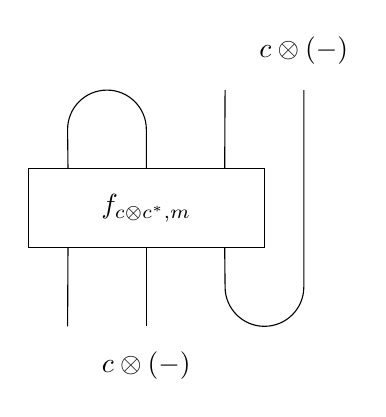
\begin{tikzpicture}
	\node (A) at (2,2) [minimum height=1cm,minimum width=3cm, draw] {$f_{c \otimes c^*,m}$};
	\draw (A.153) -- (1,3) arc (180:0:0.5cm) -- (A.90) ;
	\draw (A.27) -- (3,3.5);
	\draw (A.333) -- (3,1) arc (180:360:0.5cm) -- (4, 3.5);
	\draw (A. 270) -- (2,.5);
	\draw (A.207) -- (1,.5);
	\node at (3,4) {$\cF$};
	\node at (4,4) {$c \otimes (-)$};
	\node at (1,0) {$\cF$};
	\node at (2,0) {$c \otimes (-)$};
\end{tikzpicture}}
=
\cb{\begin{tikzpicture}
	\draw (0, 0) to [out=90, in=270] (2,3.5);
	\draw (1,0) -- (1,1) arc (180:0:.5cm) arc (180:360:.5cm) -- (3,3.5);
	\node at (2,4) {$\cF$};
	\node at (3,4) {$c \otimes (-)$};
	\node at (0,-.5) {$\cF$};
	\node at (1,-.5) {$c \otimes (-)$};
\end{tikzpicture}}
$$\end{proof}


\begin{proof}
Suppose that $\cG$ is the right adjoint to the underlying functor of $\cF$, we will show that $\cG$ naturally has the structure of a $\cC$-$\cD$-bimodule functor.  The result for left adjoints is similar.

The binatural transformation $\psi_{x,n}: x \otimes \cG(n) \rightarrow \cG(x \otimes n)$ is given by the mate:
$$x \otimes \cG(n) \rightarrow \cG \cF(x \otimes \cG(n)) \rightarrow \cG(x \otimes \cF\cG(n)) \rightarrow \cG(x \otimes n)$$
where the first map is the unit of the adjunction, the second map is the binatural transformation coming from the module functor structure on $\cF$ and the third map is the counit.  
\CSP{This looks wrong to me. It doesn't seem to match the formula. Maybe it rotates the same way as the previous one?}
\NS{I think it's fixed now.  In some sense it rotates in the opposite direction as the previous argument, but we ended up doing the lax case for one and the oplax case for the other so they're the same.  Maybe that's misleading and we should change one of them.}
\begin{center}
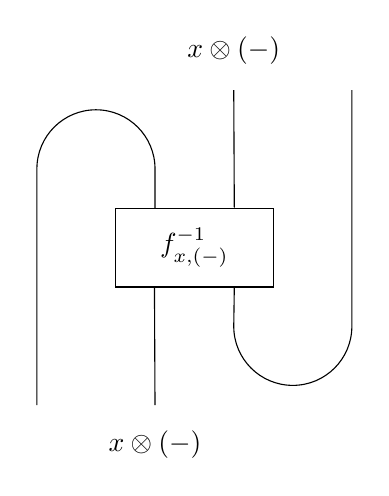
\begin{tikzpicture}
	\node (A) at (2,2) [minimum height=1cm,minimum width=2cm, draw] {$f^{-1}_{x,\cG(-)}$};
	\draw (0,0) -- (0,3) arc (180:0:0.75cm) |- (A.135);
	\draw (A.225) -- (1.5,0);
	\draw (A.45) -- (2.5,4);
	\draw (A.315) -- (2.5,1) arc (180:360:0.75cm) -- (4,4);
	\node at (2.5,4.5) {$x \otimes (-)$};
	\node at (4,4.5) {$\cG$};
	\node at (0,-0.5) {$\cG$};
	\node at (1.5, -0.5) {$x \otimes (-)$};
\end{tikzpicture}
\end{center}

Applying the previous lemma, rigidity of $\cC$ and $\cD$ guarantees that this binatural transformation is an isomorphism.  The compatibility condition is left as an exercise.
\end{proof}

\begin{remark}
If $\cC$ and $\cD$ are not rigid, the argument in the proof of this lemma only shows that the right adjoint to an (oplax) module functor has a lax module functor structure, while the left adjoint of a (lax) module functor only has an oplax module functor structure.  %This is a serious issue as the following example shows. 
\end{remark}

%\noindent From this point on we will return to our convention that all module categories are finite and all tensor categories are both rigid and finite. 




\section{The Serre automorphism and Radford's theorem} \label{sec:serre}

Traditionally topological field theories have been used as a tool to apply algebra to topology.  That is to say, a particular algebraic object yields a topological field theory which in turn gives topological invariants which can be used to prove results in topology.  However, the correspondence between algebra and topology can run the other way giving applications of topology to algebra.  A single topological calculation can be used to prove theorems in algebra by looking at the value of a bordism under a topological field theory.  In this section we give one example of this correspondence, showing that Radford's theorem on the quadruple dual functor for finite tensor categories follows from the Dirac belt trick in topology.

Here's a quick outline of the argument.  Since $\pi_1(SO(3)) \cong \mathbf{Z}/2$, there are two different $3$-framings on the interval.  We call the nontrivially $3$-framed interval the loop bordism.  Furthermore, $\pi_1(SO(3)) \cong \mathbf{Z}/2$ tells us that there's a bordism from the square of the loop bordism to the interval which we call the belt bordism (because it is the bordism traced out by the Dirac belt trick).  If $\cC$ is a separable tensor category, we can apply the local TFT attached to $\cC$ to the belt bordism.  The image of the loop bordism is called the Serre automorphism and it turns out to be closely related to the double dual.  The image of the belt bordism yields the Radford isomorphism trivializing the quadruple dual.  Thus Radford's theorem for separable tensor categories follows from the belt trick.

Note that this application does not depend on the full power of the cobordism hypothesis, as we only need to know how to interpret a few particular bordisms rather than all possible bordisms.  Looking closely at which handles appear in the belt bordism, it turns out that one can weaken the ``fully dualizable" hypothesis somewhat and still have enough maps to use the belt trick.  This version of the argument does not depend on the cobordism hypothesis and also gives a proof of Radford's theorem for non-separable finite tensor categories.


\subsection{The Serre automorphism}  \CDcomm{Move this subsection to the section on Local Field Theory in Dimension 3.}
\CSP{This Section moved to Local Field theory section}



\subsection{The Serre automorphism of a separable fusion category}

Suppose that $\cA$ is a symmetric monoidal $n$-category and that $a \in \cA$ is a fully dualizable object.  Then the image of the loop bordism gives the Serre automorphism $\cS_a: a \rightarrow a$.

We would like to make this definition more explicit.  Let $\ev : a \otimes a^{\vee} \ra 1$ and $\coev: 1 \ra a^{\vee} \otimes a$ denote the evaluation and coevaluation maps for the duality between $a \in \cA$ and its dual $a^{\vee} \in \cA$.  Let $\ev^R: 1 \ra a \otimes a^{\vee}$ be the right adjoint to $\ev$.  Let $\tau: a \otimes a \ra a \otimes a$ denote the symmetric monoidal switch.  \NS{Make sure we explain this notation somewhere earlier}

\begin{proposition}
Let $a \in \cA$ be a dualizable object of the symmetric monoidal n-category $\cA$, for $n \geq 2$.  The Serre automorphism $\cS_a : a \ra a$ is equivalent to the following composite:
\[
\cS_a \simeq (\ev \btimes \id_a) \circ (\id_{a^{\vee}} \btimes \tau) \circ (\ev^R \btimes \id_a)
\] 
\end{proposition}

We now specialize to our case of interest, namely where the object in question is a finite tensor category (which is a dualizable object in the $(3,2)$-category $\TC$).  The value of the Serre automorphism of such a tensor category was listed in a table in the previous section---we now make the calculation of the automorphism more explicit.

%\CD{Where did we establish that $\Hom_D(M,D)$ is a left/right adjoint to M, etc, and under what conditions? --- the identification of Serre depended on this!}

\begin{definition}
Suppose that $\cC$ is a finite tensor category and $\cF: \cC \rightarrow \cC$ is an automorphism of tensor categories.  Let ${}_{\langle\cF\rangle} \cC$ denote $\cC$ as a $\cC$--$\cC$ bimodule where the action is $x \cdot c \cdot y = \cF(x) \otimes c \otimes y$ with the obvious natural transformations.  
\end{definition}

\begin{theorem} \label{thm:serre}
If $\cC$ is a finite tensor category, then the Serre bimodule $\bimod{\cC}{\cS}{\cC}$ for $\cC$ is equivalent as a bimodule category to ${}_{\langle\ldd{(-)}\rangle} \cC$.
\end{theorem}

\begin{proof}
We compute $\cS_a \simeq (\ev \btimes \id_a) \circ (\id_{a^{\vee}} \btimes \tau) \circ (\ev^{*} \btimes \id_a) \simeq (\ev \boxtimes \id_a) \circ (\id_a \boxtimes (\tau_{a^\vee,a} \circ  \ev^*))$ in two steps.  

First we consider $\tau_{a^\vee,a} \circ  \ev^*$.  By Lemma \ref{lem:dual-formula-for-adjoints}, $\ev^*$ is $\cC^{\op}$ as a $\Vect$--${\cC \boxtimes \cC^{\mp}}$ bimodule where the action is given by $m\cdot (x \boxtimes y) = {}^*y \otimes m \otimes x^*$ (here we've used that the left dual in $\cC^{\mp}$ is the right dual in $\cC$).  Hence, $\tau_{a^\vee,a} \circ  \ev^*$ is $\cC^{op}$ as a $\Vect$--$\cC^{mp} \boxtimes \cC$ bimodule, where the action is given by $c \cdot (y \boxtimes x) =  {}^*y \otimes c \otimes x^*$.  Taking right duals, we see that $\tau_{a^\vee,a} \circ  \ev^*$ equivalent to $\cC$ as a $\Vect$--$\cC^{mp} \boxtimes \cC$ bimodule, where the action is given by $c \cdot (y \boxtimes x) =  {}^{**}y \otimes c \otimes x$.

Now we compose with $\ev \boxtimes \id_a$, which just turns a right $\cC^{\mp}$ action into a left $\cC$ action.  So $\cS_a$ is equivalent to $\cC$ as a  $\cC$--$\cC$ bimodule, where the action is given by $y \cdot c \cdot x=  {}^{**}y \otimes c \otimes x$.
\end{proof}

Thus the fact that $\pi_1(SO(3)) \cong \mathbb{Z}/2$ has the following consequence in $\TCsep$.

\begin{corollary}
If $\cC$ is a separable fusion category, then ${}_{\langle{}^{****}(-)\rangle} \cC \cong {}_{\langle\id\rangle} \cC$.
\end{corollary}

We would like to turn this into a statement about the functor ${}^{****}(-)$ itself.

\begin{lemma}
Suppose that $\cF$ is a $\cC$--$\cC$ bimodule equivalence $\cC \rightarrow {\langle \alpha \rangle}_\cC$, then $\cF(1)$ is invertible and $\alpha$ is naturally isomorphic as a monoidal functor to the conjugation functor $c \mapsto \cF(1) c \cF(1)^{-1}$.  
\end{lemma}
\begin{proof}
$\cF(1)$ is invertible because it generates $\cC$ as a right module category.  The natural transformation from $\alpha$ to conjugation by $\cF(1)$ is determined by the composite 
$$\alpha(c) = \alpha(c) \cF(1) \cF(1)^{-1} \mapsto \cF(c) \cF(1)^{-1} \mapsto \cF(1) c \cF(1)^{-1}$$
where the first map is the natural transformation coming from right module functor structure on $\cF$ and the second map is the natural transformation coming from the left module structure on $\cF$.  This natural isomorphism is monoidal, as required. 

\end{proof}

\begin{corollary}
The quadruple dual is equivalent to conjugation by some invertible object $X$.
\end{corollary}

Recall that not only do we know that ${}_{\langle{}^{****}(-)\rangle} \cC \cong {}_{\langle\id\rangle}\cC$, we actually have a canonical natural isomorphism given by the image of the universal belt map.  We call the image of this map the Radford isomorphism $\cR_\cC: \cC \rightarrow \cS \boxtimes_\cC \cS$.  The Radford isomorphism $\cR_\cC$ gives a canonical choice of invertible object $X = \cR(1)$ in the above corollary, and gives a canonical natural isomorphism between the quadruple dual and conjugation by the canonical invertible object $X$.

\begin{lemma} \label{lem:belt-formula}
The universal belt map is given by the following composition of basic bordisms where $p$ is the positively framed point,
\NS{We need to check conventions here for order of composition}
\begin{align*} 
\id_p &\rightarrow \id_p \circledcirc (\ev_p^R \circ \id_{p \otimes p^\vee} \circ \ev_p)  \rightarrow (\id_p \circledcirc \ev_p^R) \circ (\tau \circledcirc \id_{p^\vee}) \circ (\id_{p^\vee} \circledcirc \id_p \circledcirc \id_{p^\vee}) \circ (\tau \circledcirc \ev_p) \\
&\rightarrow (\id_p \circledcirc \ev_p^R) \circ (\tau \circledcirc \id_{p^\vee}) \circ (\id_p \circledcirc \ev_p) \circ \id_p \circ (\id_p \circledcirc \ev_p^R) \circ (\tau \circledcirc \id_{p^\vee}) \circ (\id_p \circledcirc \ev_p) = \cS_p \circ \cS_p
\end{align*}  
\end{lemma}

\begin{remark}
Note that although the universal belt map is a $2$-dimensional bordism, it does not have a $2$-framing, but only a $3$-framing.  This fact is reflected in the above explicit formula, which includes an adjoint of one of the basic $2$-morphisms.  Thus, even though it's a $2$-dimensional bordism, it requires at least part of a $3$-dimensional theory to define.  
\end{remark}

\begin{theorem} 
For a fusion category $\cC$ the canonical invertible object is trivial.
\end{theorem}
\begin{proof}
\NS{Use proof from email}
\end{proof}

\subsection{The Radford isomorphism for separable fusion categories}

\CDcomm{This section just applies the cobordism hypothesis on the belt trick.}

\subsection{The Radford isomorphism for finite tensor categories}

\CDcomm{This section is motivated by the previous, but doesn't use the CH, instead uses the categorical belt trick.}

Recall that although finite tensor categories are not fully dualizable, they are $2$-dualizable and furthermore most of the basic $3$-morphisms have adjoints.  The latter fact suggests that there should be a fully extended $3$-dimensional field theory which is only defined on certain $3$-morphisms (this is called a ``non-compact" field theory by Lurie \cite[\S4.2]{lurie-ch}).  In particular, we should expect that the $2$-framed $2$-dimensional field theory attached to a finite tensor category has a canonical descent to a $3$-framed theory.  We plan to address this in more detail in a later paper, so we will be brief in this section and not try for the strongest results.

\begin{theorem}
The $2$-framed $2$-dimensional TFT attached to a rigid finite tensor category has a canonical descent to a $3$-framed $2$-dimensional TFT given by the canonical trivialization $(-)^{****} \rightarrow D (-) D^{-1}$ where $D$ is the canonical invertible object from \cite{MR2097289}.
\end{theorem}
\begin{proof}
\NScomm{[In process.]}  %!%The main content of the proof is topological, that is using an explicit descriptions of $SO(3)$ and $SO(2)$ you can show that the data needed to turn a $2$-framed theory into a $3$-framed theory is exactly a trivialization of the square of the Serre automorphism.]}
\end{proof}

The above result is unsatisfactory in two ways.  First, it does not give a topological reason for the appearance of $3$-framings.  We would prefer to have a partially defined $3$-dimensional theory which explains the appearance of a structure group which is naturally attached to $3$-dimensional theories.  Second, it relies on a non-topological proof of Radford's theorem.  These two defects are closely related: a partially defined $3$-dimensional TFT would be automatically $3$-framed and thus would give a topological proof of Radford's theorem.  In fact, as we saw in the last section, most of the $2$-handles automatically have adjoints.  This suggests that most of the $3$-handles can be defined, in particular enough of them to give a topological proof of Radford's theorem.

It is an important philosophical point that algebraic applications of the cobordism hypothesis do not rely on the full strength of the cobordism hypothesis.  Any given application uses specific relationships between specific bordisms, and thus only relies on a very small part of the full topological field theory.  In particular, if you look at the explicit formula for the universal belt map, we don't need a full $3$-dimensional field theory, we only need that the $2$-framed saddle has an adjoint.  Thus, rather than rigorously constructing a non-compact field theory, if all we want is Radford's theorem we can just write down formulas for the particular bordisms that we need and check that those formulas work.

\begin{theorem}
If $\cC$ is a finite tensor category, then the formula from Lemma \ref{lem:belt-formula} gives an isomorphism between $\cC$ and $\cS \boxtimes_\cC \cS$.  Furthermore, under this map the image of $1$ gives a canonical invertible object $D$, and this formula gives a canonical equivalence between the quadruple dual and conjugation by $D$.
\end{theorem}
\begin{proof}
\NScomm{[We still need to work through the details here.]}
\end{proof}

Another way to think of Radford's theorem is that it states that there's an equivalence between the left Serre automorphism and the right Serre automorphism.  Recalling the definitions of these two automorphisms, that's the same as saying that the left adjoint of $\ev_a$ is canonically equivalent to the right adjoint of $\ev_a$.  This version of the statement has a generalization which again is inspired by the cobordism hypothesis but does not rely on the proof of the cobordism hypothesis.


\subsection{Sphericality and the quadruple dual}

%!% \CDcomm{Need to rephrase what is happening in this section.  Can just leave with no intro for now.}  In this section we check that our constructions from the last two subsections agree with the constructions in \cite{MR2097289}.
.%!% remove period

\CDcomm{This section contains the comparison of our Radford to ENO Radford, and applications.}

\CDcomm{[This section under construction]}

\begin{proposition}
If $\cC$ is a finite rigid tensor category, our canonical invertible agrees with the one in \cite{MR2097289}, and our Radford map agrees with the one in \cite{MR2097289}.
\end{proposition}
\begin{proof}
\NScomm{[I know how to prove this now but need to write it up.]}
\end{proof}

\begin{lemma} \label{lem:hspherical-implies-spherical}
A pivotal structure $p$ is spherical if and only if $p p^{**}$ agrees with the canonical trivialization of the quadruple dual induced by the Radford isomorphism.
\end{lemma}
\begin{proof}
\NScomm{[This can be proved by modifying the calculation in ENO where they prove that the pivotalization is spherical.]}
\end{proof}

%%%%%%


%!% Temporary document end

\bibliographystyle{alpha}
\bibliography{bibliography/bibliography}
\end{document}

%%%


\section{CD's dustbin/workbin}

\subsection{This section to be removed after comment addressed} \label{sec:pivot-struc}

\begin{conjecture}
Every oriented-$p_1$ local field theory with values in tensor categories descends to an oriented local field theory.
\end{conjecture}
\CDcomm{[9/24/11] We now know that this conjecture is false, right?  That is, it is possible to pick Morita spherical structures with nontrivial anomaly.}


\section{NS's dustbin/workbin}

The following result, which is a generalization of Radford's `$S^4$ formula' for Hopf algebras, is an important result in the theory of fusion categories. The proof in \cite{MR2183279} appeals to the fact that every fusion category is equivalent to the representation category of a weak Hopf algebra.  

\begin{theorem}[\cite{MR2183279}]
	A fusion category $\cC$ admits a canonical monoidal equivalence between the identity functor and the quadruple dual functor $\ldddd{(-)}$.
\end{theorem}

\CSP{cite which theorem of ours does this.}
We will give a new proof of this theorem based on the fact that fusion categories are fully dualizable objects in the symmetric monoidal 3-category of tensor categories (described later in this paper).

\begin{definition}
A fusion category $\cC$ is \emph{pivotal} if it admits a {\em pivotal structure}: a monoidal equivalence between the double right dual functor $\ldd{(-)}: \cC \xra{\ld{(-)}} \cC^{\mop} \xra{\ld{(-)}} \cC$ and identity functor.
\end{definition}

In other words, a fusion category is pivotal if the left dual functor $\ld{(-)}: \cC \ra \cC^{\mop}$ and the right dual functor $\rd{(-)}: \cC \ra \cC^{\mop}$ are monoidally equivalent.


\begin{definition}
	A pivotal structure is {\em spherical} if it induces a monoidal equivalence between the identity functor and the quadruple dual functor which agrees with the canonical equivalence. A fusion category is {\em spherical} if it admits a spherical pivotal structure.  
\end{definition}

\CSP{NS, can you double check this again? I get lost with the calculations.}
\begin{remark}
	It follows from \cite[Cor. 7.4]{MR2097289} that for fusion categories the above notion of spherical coincides with the usual notion: the left and right traces induced from the pivotal structure agree.
\end{remark}



\section{CSP's dustbin}

Let $A$ be a finite set. We define a strict 2-category $\lincat(A)$ as follows. Let $P(A)$ denote the powerset of $A$, and let $S$, $S'$, and $S''$ denote various disjoint subsets of $A$. The objects of $\lincat(A)$ consist of  $P(A)$-tuples of objects in $\lincat$, together with some additional data. Thus we have a finite linear category $X(S)$ for each subset $S \subseteq A$. The additional data consists of bilinear functors
\begin{align*}
		x_{S,S'}: & \; X(S) \times X(S') \to X(S \sqcup S') \\
		I: & \; \Vect \to X(\emptyset)
\end{align*}
and natural isomorphisms of multi-linear functors
\begin{align*}
		\alpha_{S, S', S''}:  & \; x_{S \sqcup S', S''}\circ (x_{S,S'} \times 1) \cong x_{S, S' \sqcup S''} \circ (1 \times x_{S', S''}) \\
		r_S: & \; x_{S, \emptyset} \circ (1 \times I)  \cong  \textrm{can}^r \\
		\ell_{S}: & \; x_{ \emptyset, S} \circ (I \times 1)  \cong  \textrm{can}^\ell
\end{align*}
where $\textrm{can}^r: X(S) \times \Vect \to X(S)$ is the canonical bilinear functor, and similarly for $\textrm{can}^\ell$. 
Moreover this data is subject to the following conditions: 
\begin{enumerate}
	\item $x_{S,S'}$ realizes $X(S \sqcup S')$ as the Deligne tensor product  $X(S) \boxtimes X(S') $, and $I$ is an isomorphism of linear categories. 
	\item $	\alpha_{S, S', S''}$ satisfies the evident pentagon identity. 
	\item $\ell_S$, $r_S$, and $\alpha_{\emptyset, S, \emptyset}$ satisfy the evident triangle identity.
\end{enumerate}

A morphism $f:X \to Y$ in $\lincat(A)$ consists of a $P(A)$-tuple of linear functors $f_S: X(S) \to Y(S)$, together with natural isomorphisms of bilinear functors $\phi_{S,S'}: y_{S,S'} \circ f_S \times f_{S'} \cong f_{S \sqcup S'} \circ x_{S,S'}$. For each triple $S$, $S'$, $S''$ of disjoint subset of $A$, the following hexagon identity holds,
\begin{equation*}
	[1 * \alpha^X_{S, S', S''}] \circ [\phi_{S \sqcup S', S''} * 1] \circ [1 *(\phi_{S, S'} \times 1)] = 
		[\phi_{S, S' \sqcup S''} * 1] \circ [1 * (1 \times \phi_{S', S''})] \circ [\alpha^Y_{S,S', S''} * 1].
\end{equation*}

A 2-morphism $\theta: f \to g$ in $\lincat(A)$ consists of a $P(A)$-tuple of linear natural transformations $\theta_S: f_S \to g_S$, such that for every pair of disjoint subsets $S$, $S'$ of $A$ the following identity holds: 
\begin{equation*}
	(\theta_{S\sqcup S'}* 1) \circ \phi^f_{S,S'} = \phi^g_{S,S'} \circ (1 * (\theta_S \times \theta_{S'})).
\end{equation*}

One readily verifies that $\lincat(A) \simeq \lincat^{\times A}$. Thus an object of $\lincat(A)$ can roughly be thought of as consisting of an $A$-tuple of linear categories. However the object of $\lincat(A)$ also includes choices of representatives for the possible Deligne tensor products of these linear categories. The assignment $A \mapsto \lincat(A)$ gives a strict functor from $\Gamma^\op \simeq \Fin_*$ to strict 2-categories, which by abuse of notation we will also denote by $\lincat$. 





\CSPcomm{
\begin{itemize}
	\item levelwise $\boxtimes$ makes $\lincat(A)$ weakly monoidal, can define tensor cats, module cats etc etc.  
\end{itemize}

\subsection{The symmetric monoidal 2-categories of tensor categories and bimodule categories}

Let $\TC(A)$ be the collection of all sextuples $(X, \otimes, \mathbf{1}, \alpha, \ell, r)$ where $X \in \lincat(A)$,  $\otimes: \Delta^*(X \boxtimes X) \to X$, $\mathbf{1}: \Vect \to X$, $\alpha$, $\ell$, $r$ are the associator and unitors, satisfying the usual conditions. 

}




%Fix a finite set $A$. This gives rise to a functor $j_A: \Delta \to \Gamma$ which sends the ordered set $[m]$ to the set $\sqcup_m A = \{ (a,i) \; | \; a \in A, \; 0 < i \leq m \} $, and sends $f: [m] \to [n]$ to the function $ (a,i) \mapsto \{ (a,j) \in \sqcup_n A \; | \; f(i-1) < j \leq f(i) \}$. Composing with $\lincat$ gives a strict simplicial 2-category. In particular for each object $X \in \lincat(\sqcup_n A)$ and each $\varphi: [m] \to [n]$ in $\Delta$, we obtain an object $\varphi^*X \in \lincat(\sqcup_m A)$.

%Another important simplicial 2-category, is the terminal simplcial 2-category, which is the constant functor with value the terminal 2-category $pt$. A semi-lax natural transformation from $pt$ to $\lincat \circ j_A$ consists of a family of objects $\{ X_n \in \lincat(\sqcup_n A)\}$ together with functors $X_\varphi: \varphi^*X_n \to X_m$ and natural isomorphisms $\phi_{\varphi, \psi}: X_\varphi \circ \varphi^* X_\psi \cong X_{\psi \varphi}$ for each $\varphi: [m] \to [n]$ and $\psi: [n] \to [p]$ in $\Delta$. These natural isomorphisms are required to satisfy the pentagon identity. There is a 2-category of such natural transformations. 

%For each $1 \leq i \leq n$, let $s_i: [1] \to [n]$ denote the {\em Segal inclusion} which maps $0\mapsto i-1$, and $1 \mapsto i$. 
%
%\begin{definition}
%	A {\em tensor category} in $\lincat(A)$ is a semi-lax natural transformation $X: pt \to \lincat \circ j_A$ such that the functors $X_{s_i}: s_i^*X_n \to X_1$ are equivalences. 
%\end{definition}
%
%In the case that $A = (1) = \{1\}$, this is essentially equivalent to the usual notion of a tensor category. 








%There is a functor $\varphi:\Delta \to \Gamma$, which sends $[m]$ to the set $(m) = \{ 1, 2, \dots, m\}$, and sends $f: [m] \to [n]$ to the function $\varphi_f: i \in (m) \mapsto \{ j \in (n) \; | \: f(i-1) < j \leq f(i) \}$.


%The first significant advantage of $n$-fold Segal categories follows from the fact that the homotopy fiber product over a discrete base, for example $X_m \times_{X_0}^h X_n$ when $X$ is an $n$-fold Segal category, agrees with the ordinary fiber product. Thus we many avoid a lengthly discussion of the model structure of $n$-fold complete Segal spaces and work directly with ordinary fiber products.

%We must also identify the weak equivalences between $n$-fold Segal categories. These admit a fairly direct inductive description in terms of the homotopy category $hX$ of an $n$-fold Segal category.



%-----


%The {\em homotopy pull-back} of $n$-fold simplicial spaces may be inductively defined as follows. For $0$-fold simplicial spaces a homotopy pull-back is a homotopy pull-back in the standard model structure on simplicial sets. For general $n$-fold simplicial spaces $W$, $X$, $Y$, and $Z$, a diagram 
%\begin{center}
%\begin{tikzpicture}
%	\node (LT) at (0, 1.5) {$W$};
%	\node (LB) at (0, 0) {$X$};
%	\node (RT) at (2, 1.5) {$Y$};
%	\node (RB) at (2, 0) {$Z$};
%	\draw [->] (LT) -- node [left] {$$} (LB);
%	\draw [->] (LT) -- node [above] {$$} (RT);
%	\draw [->] (RT) -- node [right] {$$} (RB);
%	\draw [->] (LB) -- node [below] {$$} (RB);
%	%\node at (0.5, 1) {$\ulcorner$};
%	%\node at (1.5, 0.5) {$\lrcorner$};
%\end{tikzpicture}
%\end{center}
%is a homotopy pull-back diagram if and only if for each $n$ the diagram 
%\begin{center}
%\begin{tikzpicture}
%	\node (LT) at (0, 1.5) {$W_n$};
%	\node (LB) at (0, 0) {$X_n$};
%	\node (RT) at (2, 1.5) {$Y_n$};
%	\node (RB) at (2, 0) {$Z_n$};
%	\draw [->] (LT) -- node [left] {$$} (LB);
%	\draw [->] (LT) -- node [above] {$$} (RT);
%	\draw [->] (RT) -- node [right] {$$} (RB);
%	\draw [->] (LB) -- node [below] {$$} (RB);
%	%\node at (0.5, 1) {$\ulcorner$};
%	%\node at (1.5, 0.5) {$\lrcorner$};
%\end{tikzpicture}
%\end{center}
%is a homotopy pull-back diagram of $(n-1)$-fold simplicial spaces. Thus homotopy fiber products are computed `levelwise'. In particular if $Z$ is a discrete $n$-fold simplicial space, then the homotopy fiber product is levelwise homotopy equivalent to the usual fiber product. 

	
	
%	We now inductively define a class of objects called {\em $n$-fold Segal spaces} as well as a collection of maps of $n$-fold Segal spaces called {\em weak equivalences}. For $0$-fold simplicial spaces Segal spaces are the Kan complexes. The weak equivalences between $0$-fold simplicial spaces are the weak equivalences of simplicial sets.  
	

%\CSPcomm{[There is a model category of $\Gamma$-$n$-fold complete Segal spaces which models symmetric monoidal $(\infty, n)$-categories]. The is a completion functor (fibrant replacement), so it is enough to produce a $\Gamma$-$n$-fold simplicial space. We produce a Segal one.}



\subsection{Tensor products and colimits of linear categories} \label{sec:tc-tensorprod}

\begin{definition}
\CDcomm{[Definition of a tensor category, include all the conditions to be an object of the 3-category, ie indemp comp, etc.]}
\end{definition}

\begin{definition} \label{def:colim}
\CDcomm{[colimits in the 2-category of (appropriate) linear categories]}
\end{definition}


We will have occasion to use both the opposite of a tensor category, and the monoidal opposite of a tensor category; we establish notation to distinguish them.  

\subsection{Tensor category bimodules and bimodule composition} \label{sec:tc-bimod}


\begin{definition}
\CDcomm{[Definition of bimodules between tensor categories]}
\end{definition}


\begin{definition}
Let $A$, $B$, and $C$ be tensor categories, and let $\bimod{A}{M}{B}$ and $\bimod{B}{N}{C}$ be bimodules.  The ``precomposite bimodule" $\bimod{A}{M \otimes_B N}{C}$ is the colimit of the three-stage two-sided bar construction:
\begin{equation} \nn
\bimod{A}{M \otimes_B N}{C} := \colim \left( M \dtimes A \dtimes A \dtimes N \righttriplearrows M \dtimes A \dtimes N \rightdoublearrows M \dtimes N \right)
\end{equation}
\end{definition}

\begin{remark} \CD{This remark is not written very precisely or correctly yet---should be fixed after the Deligne tensor is spelled out earlier on.}
By applying definition~\ref{def:colim}, one can write out explicitly the bimodule $\bimod{A}{M \otimes_B N}{C}$ given by the above colimit of the three-stage two-sided bar construction.  There is however an equivalent bimodule $\bimod{A}{M \otimes_B' N}{C}$ that admits a more compact description, as follows.  The objects of $\bimod{A}{M \otimes_B' N}{C}$ are the objects $m \otimes n$ of the tensor product $M \dtimes N$.  The morphisms are of two kinds: (m1) a morphism $\phi \otimes \psi : m \otimes n \ra m' \otimes n'$ for each pair of morphisms $\phi: m \ra m'$ in $M$ and $\psi: n \ra n'$ in $N$; (m2) a morphism $t_a : ma \otimes n \ra m \otimes an$ for each \CDcomm{triple $(m,a,n)$ ... }.  These morphisms are subject to the two relations: (r1) for each \CDcomm{triple $(\phi, \epsilon, \psi)$}, the composite $ma \otimes n \ra m \otimes an \ra m' \otimes a' n'$ equals the composite $ma \otimes n \ra m' a' \otimes n' \ra m' \otimes a' n'$; (r2) the composite $(ma)b \otimes n \ra ma \otimes bn \ra m \otimes a(bn)$ equals the composite $(ma)b \otimes n \ra m(ab) \otimes n \ra m \otimes (ab)n \ra m \otimes a(bn)$.
\end{remark} % cf ENOII "Explicit description 1"



\begin{definition}
Let $A$, $B$, and $C$ be tensor categories, and let $\bimod{A}{M}{B}$ and $\bimod{B}{N}{C}$ be bimodules.  The composite bimodule $\bimod{A}{M \dtimes_B N}{C}$ is the idempotent completion of the precomposite bimodule:
\begin{equation} \nn
\bimod{A}{M \dtimes_B N}{C} := \IC \left( \bimod{A}{M \otimes_B N}{C} \right)
\end{equation}
\end{definition}

\begin{example}
\CDcomm{$\Vect \dtimes_{\Vect[\ZZ/2]} \Vect$ is $\Vect \oplus \Vect$, [cf ENOII "Example 1 (cont):"]}
\end{example}

%%%

\begin{proposition} \CD{Not sure whether we need this prop or where it best belongs.}
Let $A$ be a \CDcomm{...} monoidal indempotent complete linear category, and let $M$ and $N$ be $A$-modules.  If $N$ is idempotent complete, then $\Hom_A(M,N)$ is idempotent complete.
\end{proposition}

\begin{corollary}
For $A$ and $B$ tensor categories, and $M$ an $A$-$B$ bimodule, if $\bimod{A}{M}{B}$ has a right adjoint, then that right adjoint is $\bimod{B}{\Hom_A(M,A)}{A}$.
\end{corollary}

\begin{proof}
\CDcomm{[Proof sketch of corollary at ENOII "Next steps on adjoints of 1-morphisms".]}
\end{proof}


\section{Old 2d examples section}

\CSPcomm{
Some values for circles. With framing: $-1$, $0$, $+1$. 
\begin{align*}
	\cZ(\cC) & = \ev^L \boxtimes_{\cC \boxtimes \cC^\mp} \ev \cong \Fun_{\cC \boxtimes \cC^\mp}(\cC,\cC) \\
	\cT(\cC) & = \coev \boxtimes_{\cC^\mp \boxtimes \cC} \tau \boxtimes_{\cC \boxtimes \cC^\mp} \ev \\
	\overline{\cZ}(\cC) & = \ev^R \boxtimes_{\cC \boxtimes \cC^\mp} \ev \cong \Fun(\cC, \Vec) \boxtimes_{\cC \boxtimes \cC^\mp} \cC.
\end{align*}
}


\subsubsection{The Serre automorphism and convention invariance}

. % remove period
\CSPcomm{This subsection does several things. 
\begin{itemize}
	\item It gives an invariance lemma which allows us, for example, to compute the value of framed circles using distinct choices of evaluations, etc. (This is key to being able to write down enough pants to compute four interesting tori).
	\item It computes the Serre in the $\cC^\mp$ convention
	\item It gives the $\cC^\op$-convention and shows how the Serre is more symmetric in that convention. 
\end{itemize}
}

\CSPcomm{these remarks moved here, they will become part of the discussion}

\begin{remark}
The above formulas for intervals have a somewhat unsatisfying assymmetry, where two intervals which look very similar (say with no twists) have answers which look rather different (say one is $\cC$ and the other $\cC^*$).  This comes from our choices of preferred duality between a positively framed point and a negatively framed one.  We could just as well have fixed intervals which rotate clockwise instead of counterclockwise and we would get values which were assymetric in the other direction.  

It is also possible to pick conventions that make the formulas more symmetric but at the cost of not identifying all positively framed points with $\cC$, but instead identifying some of them with $\cC^{\mop}$.  Similarly instead of identifying all negatively framed points with $\cC^\mp$ we can identify some with $\cC^\op$ instead.  One very natural choice is the following.

TABLE:
Values of four points
Values of some non-bending intervals (agreeing with 1-dimension)
Values of some bending intervals
Value of Serre

From this point of view the appearance of the double dual looks more natural.  Namely, rotation by $180$-degrees always twists by a single dual, so $360$-degree rotation twists by a double dual.  Note however, that this point of view does not simplify the calculation of these values, it only makes the answer look less surprising.
\end{remark}

\subsubsection{Values for pants}

Using these formulas it is possible to compute the values of certain more complicated $2$-bordisms.  For example, we have the following formula for the pair of pants.

IMAGE

Note that there are actually a $\mathbb{Z}\times \mathbb{Z}$ torsor of different $2$-framed pairs of pants.  We give one example.

IMAGE

\CSPcomm{We will actually give four examples, which become representantives of the four 3-framed pants}

\CSP{This section should mention that the center $\cZ(\cC)$ is naturally a braided monoidal category.
}

\subsubsection{Values for copants}

. %remove period
\CSPcomm{Mention how the dual center $\overline{\cZ}(\cC)$ is naturally a braided comonoidal category.}

\subsubsection{Values for Tori}

Similarly one can compute the values of $2$-framed surfaces.  Note that there is no $2$-framing on the sphere, while there are many $2$-framings of the torus.  Since our theories are actually $3$-framed, we do not go into detail on the values of $2$-framed surfaces here.
 
\CSP{Here the equation for the tori is just given in terms of the pants, but the exact value is not computed until the last section when we are in the separable setting.}


\NScomm{This is the end of the current outline of the section.  The material below will be canibalized and moved to the appropriate locations above.} 
 
We will give two different representatives.  The first choice corresponds directly to the proofs in the previous subsection, while the second choice is clearly equivalent to the first but is more symmetric.


Table~\ref{table-points} lists four standard 2-framed 0-manifolds along with their associated invariants.
\begin{table}[ht]
\begin{tabular}{c|l|l}
\cb{
\begin{tikzpicture}
\filldraw (0,0) circle (\pointrad);
\begin{pgfonlayer}{background}
\draw[->,outstyle] (0,0) -- +(0:\arrowlength) node[anchor=south west,inner sep=1pt] {\tiny 1};
\draw[->,outstyle] (0,0) -- +(90:\arrowlength) node[anchor=south west,inner sep=1pt] {\tiny 2};
\end{pgfonlayer}
\end{tikzpicture}
}
& $\cC$ & $\cC$ \\[6pt]
\cb{
\begin{tikzpicture}
\filldraw (0,0) circle (\pointrad);
\begin{pgfonlayer}{background}
\draw[->,outstyle] (0,0) -- +(180:\arrowlength) node[anchor=south east,inner sep=1pt] {\tiny 1};
\draw[->,outstyle] (0,0) -- +(90:\arrowlength) node[anchor=south east,inner sep=1pt] {\tiny 2};
\end{pgfonlayer}
\end{tikzpicture}
}
& $\cC^\mp$ & $\cC^\mp$ \\[6pt]
\cb{
\begin{tikzpicture}
\filldraw (0,0) circle (\pointrad);
\begin{pgfonlayer}{background}
\draw[->,outstyle] (0,0) -- +(0:\arrowlength) node[anchor=north west,inner sep=1pt] {\tiny 1};
\draw[->,outstyle] (0,0) -- +(-90:\arrowlength) node[anchor=north west,inner sep=1pt] {\tiny 2};
\end{pgfonlayer}
\end{tikzpicture}
}
& $\cC^\mp$& $\cC^\op$ \\[6pt]
\cb{
\begin{tikzpicture}
\filldraw (0,0) circle (\pointrad);
\begin{pgfonlayer}{background}
\draw[->,outstyle] (0,0) -- +(180:\arrowlength) node[anchor=north east,inner sep=1pt] {\tiny 1};
\draw[->,outstyle] (0,0) -- +(-90:\arrowlength) node[anchor=north east,inner sep=1pt] {\tiny 2};
\end{pgfonlayer}
\end{tikzpicture}
}
& $\cC$ & $\cC^\mop$
\end{tabular}
\caption{Invariants associated to 2-framed 0-manifolds.} \label{table-points}
\end{table} 
Notice that the first and fourth (and similarly the second and third) are equivalent, but not canonically equivalent, framed manifolds; their invariants are thus also equivalent, but not canonically so.  \NS{Say something more here}

%Of course, one could write down an equivalent TFT where all positive points are sent to $\cC$ and all negative points are sent to $\cC^{\mp}$, but this would break certain symmetries (in particular, you need to choose which way to identify the second and third points above, and there are two such natural choices).

A generating collection of 2-framed 1-manifolds have invariants as listed in Table~\ref{table-intervals}.
\begin{table}[ht]
\begin{tabular}{c|c|cl}
\cb{
\begin{tikzpicture}
\draw[linestyle,fuzzright] (0,0) arc (-90:90:\smcirclerad);
\end{tikzpicture}
}
& $\bimod{\cC \btimes \cC^\mp}{\cC}{\Vec}$ 
& $\bimod{\cC \btimes \cC^\op}{\cC}{\Vec}$ 
& via $\cC^\op \xra{(-)^*} \cC^\mp$ \\
%
\cb{
\begin{tikzpicture}
\draw[linestyle,fuzzright] (0,0) arc (90:270:\smcirclerad);
\begin{pgfonlayer}{background}
	\draw[->,outstyle] (0,0) -- +(0:\arrowlength);
	\draw[->,outstyle] (0,-2*\smcirclerad) -- +(0:\arrowlength);
\end{pgfonlayer}
\end{tikzpicture}
}
& $\bimod{\Vec}{\Fun_{\cC \boxtimes \cC^\mp}(\cC,\cC \boxtimes \cC^\mp)}{\cC \btimes \cC^\mp}$
& $\bimod{\Vec}{\cC}{\cC \btimes \cC^\op}$ 
& via $\cC^\op \xra{{}^*(-)} \cC^\mp$ \\
%
\cb{
\begin{tikzpicture}
\draw[linestyle,fuzzleft] (0,0) arc (-90:90:\smcirclerad);
\end{tikzpicture}
} 
& $\bimod{\cC^\mp \btimes \cC}{\Fun_{}(\cC,\Vec)}{\Vec}$
& $\bimod{\cC^\op \btimes \cC}{\cC}{\Vec}$ 
& via $\cC^\op \xra{{}^*(-)} \cC^\mp$ \\
\cb{
\begin{tikzpicture}
\draw[linestyle,fuzzleft] (0,0) arc (90:270:\smcirclerad);
\begin{pgfonlayer}{background}
	\draw[->,outstyle] (0,0) -- +(0:\arrowlength);
	\draw[->,outstyle] (0,-2*\smcirclerad) -- +(0:\arrowlength);
\end{pgfonlayer}
\end{tikzpicture}
}
& $\bimod{\Vec}{\cC}{\cC^\mp \btimes \cC}$ 
& $\bimod{\Vec}{\cC}{\cC^\op \btimes \cC}$ 
& via $\cC^\op \xra{(-)^*} \cC^\mp$ \\
\cb{
\begin{tikzpicture}
\draw[linestyle,fuzzright] 
(.7,0) to [out=180, in=20] (0,-.1)
	to [looseness=1.6, out=-160, in=180] (0,-.4)
	to [looseness=1.6, out=0, in=-20] (0,-.1)
	to [out=160, in=0] (-.7,0);
\begin{pgfonlayer}{background}
	\draw[->,outstyle] (.7,0) -- +(0:\arrowlength);
\end{pgfonlayer}
\end{tikzpicture}
} 
& ---
& $\bimod{\cC}{\cC}{\cC}$ & via $\cC_{\text{in}} \xra{{}^{**}(-)} \cC$\\
\cb{
\begin{tikzpicture}
\draw[linestyle,fuzzright] 
(.7,0) to [out=180, in=-20] (0,.1)
	to [looseness=1.6, out=160, in=180] (0,.4)
	to [looseness=1.6, out=0, in=20] (0,.1)
	to [out=-160, in=0] (-.7,0);
\begin{pgfonlayer}{background}
	\draw[->,outstyle] (.7,0) -- +(0:\arrowlength);
\end{pgfonlayer}
\end{tikzpicture}
}
& ---
& $\bimod{\cC}{\cC}{\cC}$ & via $\cC_{\text{in}} \xra{(-)^{**}} \cC$\\
\cb{
\begin{tikzpicture}
\draw[linestyle,fuzzleft] 
(.7,0) to [out=180, in=20] (0,-.1)
	to [looseness=1.6, out=-160, in=180] (0,-.4)
	to [looseness=1.6, out=0, in=-20] (0,-.1)
	to [out=160, in=0] (-.7,0);
\begin{pgfonlayer}{background}
	\draw[->,outstyle] (.7,0) -- +(0:\arrowlength);
\end{pgfonlayer}
\end{tikzpicture}
}
& ---
& $\bimod{\cC^\op}{\cC^\op}{\cC^\op}$ & via $\cC^\op_{\text{in}} \xra{{}^{**}(-)} \cC^\op$\\
\cb{
\begin{tikzpicture}
\draw[linestyle,fuzzleft] 
(.7,0) to [out=180, in=-20] (0,.1)
	to [looseness=1.6, out=160, in=180] (0,.4)
	to [looseness=1.6, out=0, in=20] (0,.1)
	to [out=-160, in=0] (-.7,0);
\begin{pgfonlayer}{background}
	\draw[->,outstyle] (.7,0) -- +(0:\arrowlength);
\end{pgfonlayer}
\end{tikzpicture}
}
& ---
& $\bimod{\cC^\op}{\cC^\op}{\cC^\op}$ & via $\cC^\op_{\text{in}} \xra{(-)^{**}} \cC^\op$\\
\end{tabular}
\caption{Invariants associated to 2-framed intervals.} \label{table-intervals}
\end{table}
Throughout that table, the actions not specifically described are the naive actions.  In the first four cases, the indicated map is a tensor functor to $\cC^\mp$, therefore specifies a left action of $\cC^\op$ on $\cC$ via the natural left action of $\cC^\mp$ on $\cC$, which is to say the natural right action of $\cC$ on $\cC$.  In next set of four cases, the indicated map specifies the left action.  

\begin{remark} \label{remark-altintervals}
Though the invariants listed in Table~\ref{table-intervals} represent the most natural choices, it is possible to modify these invariants up to equivalence into less natural and less symmetrical, but sometimes more computationally convenient, forms.  For example, we may associate the invariant $\cC^\mp$ to the point
\cb{
\begin{tikzpicture}
\filldraw (0,0) circle (\pointrad);
\begin{pgfonlayer}{background}
\draw[->,outstyle] (0,0) -- +(0:\arrowlength) node[anchor=north west,inner sep=1pt] {\tiny 1};
\draw[->,outstyle] (0,0) -- +(-90:\arrowlength) node[anchor=north west,inner sep=1pt] {\tiny 2};
\end{pgfonlayer}
\end{tikzpicture}
}
rather than $\cC^\op$ as we did before.  Given that choice, we may associate the bimodule ${}_\Vec \cC_{\cC \btimes \cC^\mp}$, with the naive action, to the bordism
\cb{
\begin{tikzpicture}
\draw[linestyle,fuzzright] (0,0) arc (90:270:\smcirclerad);
\begin{pgfonlayer}{background}
	\draw[->,outstyle] (0,0) -- +(0:\arrowlength);
	\draw[->,outstyle] (0,-2*\smcirclerad) -- +(0:\arrowlength);
\end{pgfonlayer}
\end{tikzpicture}
}.
At the same time we associate the invariant ${}_{\cC^\mp \btimes \cC} \cC_{\Vec}$, again with the naive action, to the bordism
\cb{
\begin{tikzpicture}
\draw[linestyle,fuzzleft] (0,0) arc (-90:90:\smcirclerad);
\end{tikzpicture}
}.
Given these choices, the bordism
\cb{
\begin{tikzpicture}
\draw[linestyle,fuzzright] (0,0) arc (-90:90:\smcirclerad);
\end{tikzpicture}
}
is forced to have as invariant the bimodule ${}_{\cC \btimes \cC^\mp} \cC_\Vec$, where the action of $\cC^\mp$ is the naive action precomposed with the tensor functor $\cC^\mp \xra{(-)^{**}} \cC^\mp$.  That bimodule is equivalent to the bimodule $\Fun_{\cC \btimes \cC^\mp}(\cC,\cC \btimes \cC^\mp)$ with the naive actions.  Similarly the bordism
\cb{
\begin{tikzpicture}
\draw[linestyle,fuzzleft] (0,0) arc (90:270:\smcirclerad);
\begin{pgfonlayer}{background}
	\draw[->,outstyle] (0,0) -- +(0:\arrowlength);
	\draw[->,outstyle] (0,-2*\smcirclerad) -- +(0:\arrowlength);
\end{pgfonlayer}
\end{tikzpicture}
}
is forced to have as invariant the bimodule ${}_{\Vec} \cC_{\cC^\mp \btimes \cC}$, where the action of $\cC^\mp$ is the naive action precomposed with again the tensor functor $\cC^\mp \xra{(-)^{**}} \cC^\mp$.  That bimodule is equivalent to the bimodule $\Fun_{\Vec}(\cC,\Vec)$ with the naive actions.
\end{remark}

These generators can be combined into various closed manifolds, such as those depicted in Table~\ref{table-circles}.
\begin{table}[ht]
\begin{tabular}{c|cl|cl}
\cb{
\begin{tikzpicture}
\draw[linestyle,fuzzright] (0,0) circle (\smcirclerad);
\end{tikzpicture}
}
& $\cC \btimes_{\cC \btimes \cC^\mp} \cC$ & via $\cC^\mp \xra{(-)^{**}} \cC_2^\mp$ & $\Fun_{\cC \btimes \cC^\mp}(\cC,\cC)$ & via $\cC^\mp \xra{\id} \cC_2^\mp$ \\
%
\cb{
\begin{tikzpicture}
\draw[linestyle,fuzzleft] (0,0) circle (\smcirclerad);
\end{tikzpicture}
}
& $\cC \btimes_{\cC^\mp \btimes \cC} \cC$ & via $\cC^\mp \xra{{}^{**}(-)} \cC_2^\mp$ & $\Fun_{\cC \btimes \cC^\mp}(\cC,\cC)$ & via $\cC^\mp \xra{(-)^{****}} \cC_2^\mp$ \\
%
\cb{
\begin{tikzpicture}
\draw[linestyle,fuzzleft,looseness=2]
(0,.5) to [out=0, in=10] (0,0)
	to [out=-170, in=180] (0,-.5)
	to [out=0, in=-10] (0,0)
	to [out=170, in=180] (0,.5);
\end{tikzpicture}
}
& $\cC \btimes_{\cC \btimes \cC^\mp} \cC$ & via $\cC^\mp \xra{\id} \cC_2^\mp$ & $\Fun_{\cC \btimes \cC^\mp}(\cC,\cC)$ & via $\cC^\mp \xra{(-)^{**}} \cC_2^\mp$ \\
%
\cb{
\begin{tikzpicture}
\draw[linestyle,fuzzleft]
(.5,0) to [out=-90, in=-20] (0,-.4)
	to [looseness=1.6, out=160, in=180] (0,-.1)
	to [looseness=1.6, out=0, in=20] (0,-.4)
	to [out=-160, in=-90] (-.5,0)
	.. controls (-.5,.66) and (.5,.66) .. (.5,0);
\end{tikzpicture}
}
& $\cC \btimes_{\cC \btimes \cC^\mp} \cC$ & via $\cC^\mp \xra{(-)^{****}} \cC_2^\mp$ & $\Fun_{\cC \btimes \cC^\mp}(\cC,\cC)$ & via $\cC^\mp \xra{{}^{**}(-)} \cC_2^\mp$ \\
%
\cb{
\begin{tikzpicture}
\draw[linestyle,fuzzright]
(.5,0) to [out=-90, in=-20] (0,-.4)
	to [looseness=1.6, out=160, in=180] (0,-.1)
	to [looseness=1.6, out=0, in=20] (0,-.4)
	to [out=-160, in=-90] (-.5,0)
	.. controls (-.5,.66) and (.5,.66) .. (.5,0);
\end{tikzpicture}
}
& $\cC \btimes_{\cC^\mp \btimes \cC} \cC$ & via $\cC^\mp \xra{{}^{****}(-)} \cC_2^\mp$ & $\Fun_{\cC \btimes \cC^\mp}(\cC,\cC)$ & via $\cC^\mp \xra{(-)^{******}} \cC_2^\mp$ 
\end{tabular}
\caption{Invariants associated to 2-framed circles.} \label{table-circles}
\end{table}
%
\CD{Add remark about the invariants of the circles in the non-rigid case.}
The middle and right columns present two different, equivalent, formulations of the associated invariants.  For these manifolds, one can of course write the invariants directly as composites using the preceding elementary pieces, resulting in expressions involving $\cC^\op$.  We find it more convenient to think of these algebraic invariant in terms of $\cC^\mp$, as discussed in the above remark, and so have reexpressed the invariants in those terms.  In these expressions, the indicated map specifies the action of the $\cC^\mp$ factor on the second copy of $\cC$, and is therefore written as a tensor functor into ``$\cC_2^\mp$".  These five circle invariants may be briefly denoted as $\cT^{**}(\cC)$, ${}^{**}\cT(\cC)$, $\cT(\cC)$, $\cT^{****}(\cC)$, and ${}^{****}\cT(\cC)$ respectively---these expressions dervie their names from the invariants in the first column.  The invariant $\Fun_{\cC \btimes \cC^\mp}(\cC,\cC)$ in the first row is called the Drinfeld center of $\cC$ and is often denoted $\cZ(\cC)$.  Computing the invariants in the right column makes use of Theorem~\ref{thm:evcoev} and Remark~\ref{remark-altintervals} above, as well as Lemma~\ref{Lma:FunctorsAsATensorPdt} and Remark~\ref{remark-tensorasfunctors}.

In Table~\ref{table-discs}, we record the invariants associated to 2-framed discs. 
\begin{table}[ht] 
\begin{tabular}{c|l}
\cb{
\begin{tikzpicture}
\filldraw[linestyle,fuzzright,fill=\fillcolor] (0,0) circle (\circlerad);
\end{tikzpicture}
}
& $\Vec \xra{k \mapsto \id} {\Fun_{\cC \boxtimes \cC^{\mp}}(\cC,\cC)}$ \\
%
\cb{
\begin{tikzpicture}
\filldraw[linestyle,fill=\fillcolor] 
	(0,0) .. controls (.25,.25) and (.75,.25) .. (1,0)
		.. controls (.75,.25) and (.75,.75) .. (1,1)
		.. controls (.75,.75) and (.25,.75) .. (0,1)
		.. controls (.25,.75) and (.25,.25) .. (0,0);
\draw[linestyle,fuzzright]
	(0,0) .. controls (.25,.25) and (.75,.25) .. (1,0);
\draw[linestyle,fuzzleft]
	(0,1) .. controls (.25,.75) and (.75,.75) .. (1,1);
\begin{pgfonlayer}{background}
	\draw[->,outstyle] (1,1) -- +(45:\arrowlength);
	\draw[->,outstyle] (1,0) -- +(-45:\arrowlength);
\end{pgfonlayer}
\end{tikzpicture}
}
& $\Fun_{\cC \btimes \cC^\mp}(\cC,\cC \btimes \cC^\mp) \btimes \cC \xra{\mathrm{eval}} \cC \btimes \cC^\mp$ \\
%
\cb{
\begin{tikzpicture}
\filldraw[linestyle,fill=\fillcolor] 
	(0,0) .. controls (.25,.25) and (.75,.25) .. (1,0)
		.. controls (.75,.25) and (.75,.75) .. (1,1)
		.. controls (.75,.75) and (.25,.75) .. (0,1)
		.. controls (.25,.75) and (.25,.25) .. (0,0);
\draw[linestyle, fuzzleft]
	(0,0) .. controls (.25,.25) and (.25,.75) .. (0,1);
\draw[linestyle, fuzzright]
	(1,0) .. controls (.75,.25) and (.75,.75) .. (1,1);
\begin{pgfonlayer}{background}
	\draw[->,outstyle] (1,1) -- +(45:\arrowlength);
	\draw[->,outstyle] (1,0) -- +(-45:\arrowlength);
\end{pgfonlayer}
\end{tikzpicture}
}
& $\cC^\mp \btimes \cC \xra{1 \btimes 1 \mapsto \id} \Fun_{\Vec}(\cC,\cC)$ \\
%
\cb{
\begin{tikzpicture}
\filldraw[linestyle,fill=\fillcolor] (0,0) circle (\circlerad);
\end{tikzpicture}
}& $\Fun_{\Vec}(\cC,\Vec) \btimes_{\cC \btimes \cC^\mp} \cC \xra{\mathrm{eval}} \Vec$
\end{tabular}
\caption{Invariants associated to 2-framed discs.} \label{table-discs}
\end{table}

In Table~\ref{table-surfaces}, we record the invariants associated to certain 2-framed surfaces.

\begin{table}[ht] 
\begin{tabular}{c|cl}
\cb{
\begin{tikzpicture}
\filldraw[linestyle,fuzzright,fill=\fillcolor] (0,0) circle (\circlerad);
\filldraw[linestyle,fill=white] (-.4*\circlerad,0) circle (.22*\circlerad);
\filldraw[linestyle,fill=white] (.4*\circlerad,0) circle (.22*\circlerad);
\end{tikzpicture}
}
& $\Fun_{\cC \btimes \cC^\mp}(\cC,\cC) \btimes \Fun_{\cC \btimes \cC^\mp}(\cC,\cC) \xra{\alpha \btimes \beta \mapsto \alpha\beta} \Fun_{\cC \btimes \cC^\mp}(\cC,\cC)$ & % Here \alpha \beta is written with functional composition order; that is do \beta first, then do \alpha.
\end{tabular}
\caption{Invariants associated to 2-framed surfaces.} \label{table-surfaces}
\end{table}



\CDcomm{Can add to this table: annulus with fuzz out fuzz out; annulus with no fuzz; torus with any framing it is sane to draw ...}
\NScomm{Should we explain what happens in the exact tensor product but not rigid case?}
\CSPcomm{
[This is a  great spot to explain the 2D TQFT values for some of the low-dimensional cobordisms. I guess that in principle we have invertible 3D cobordisms e.g. the diffeos of the pants which induces the braiding on the center of the finite tensor category.]
}

\vspace{0.5cm}




%% The Bibliography
\bibliographystyle{alpha}
\bibliography{dtcbib}


\end{document}
